\documentclass[11pt,letterpaper]{article}
\usepackage[utf8]{inputenc}
\usepackage[provide=*,english]{babel}
\usepackage{amsmath,amssymb,amsfonts}
\usepackage[margin=2.5cm]{geometry}
\usepackage{fancyhdr}
\usepackage{enumitem}
\usepackage[most]{tcolorbox}
\usepackage{xcolor}
\usepackage{needspace}
\usepackage{tikz}
\usetikzlibrary{arrows.meta}
\usepackage{caption}
\captionsetup{font=small,labelfont={bf,color=orangeacc}}
\tikzset{vec/.style={-{Stealth[length=2mm]},thick,orangeacc},
axis/.style={-{Stealth[length=1.5mm]},graymuted},
level/.style={graymuted!65,thin}}
% Non-floating visual panels remain beside their conceptual discussion.
\newenvironment{intuitionfigure}{\par\medskip\noindent\begin{minipage}{\linewidth}\centering}{\end{minipage}\par\medskip}

\usepackage{tabularx,booktabs,array}

\definecolor{blackmain}{HTML}{1A1A1A}
\definecolor{orangeacc}{HTML}{E65C00}
\definecolor{creambg}{HTML}{FBF8F1}
\definecolor{orangebg}{HTML}{FFF4EB}
\definecolor{graymuted}{HTML}{7A746E}
\definecolor{pureblack}{HTML}{0D0D0D}

\setlength{\headheight}{24pt}
\pagestyle{fancy}
\fancyhf{}
\fancyhead[L]{\textcolor{blackmain}{\textbf{\small Mathematical Methods I}}}
\fancyhead[R]{\textcolor{orangeacc}{\textbf{\small Differential operators}}}
\fancyfoot[C]{\textcolor{graymuted}{\thepage}}
\renewcommand{\headrulewidth}{0.8pt}
\renewcommand{\headrule}{\hbox to\headwidth{\color{orangeacc}\leaders\hrule height \headrulewidth\hfill}}
\setlist[itemize]{label={\small\textcolor{orangeacc}{$\blacksquare$}},leftmargin=1.6em}
\setlist[enumerate]{label={\textcolor{orangeacc}{\arabic*.}},leftmargin=1.8em}

\newcommand{\manualsection}[1]{%
  \Needspace{13\baselineskip}%
  \vspace{0.35cm}\par\noindent{\Large\bfseries\color{blackmain} #1}\par\nobreak
  \noindent{\color{orangeacc}\rule{\linewidth}{1.4pt}}\par\nobreak\vspace{0.15cm}}
\newcommand{\manualsubsection}[1]{%
  \Needspace{6\baselineskip}%
  \par\vspace{0.2cm}\noindent{\bfseries\color{orangeacc} #1}\par\nobreak\vspace{0.12cm}}
\newtcolorbox{infobox}[2][orangeacc]{
  enhanced,colback=creambg,colframe=#1!90!black,boxrule=1pt,arc=2mm,
  left=9pt,right=9pt,top=5pt,bottom=5pt,before skip=7pt,after skip=7pt,
  before upper={\textbf{\color{#1!95!black}\large #2}\par\nobreak
    {\color{#1!50}\rule{\linewidth}{0.6pt}}\par\nobreak\smallskip}}
\newtcolorbox{examplebox}[1]{
  enhanced,colback=orangebg,colframe=orangeacc!85!black,boxrule=1pt,arc=2mm,
  left=9pt,right=9pt,top=5pt,bottom=5pt,before skip=7pt,after skip=7pt,
  before upper={\textbf{\color{orangeacc!95!black}\large #1}\par\nobreak
    {\color{orangeacc!40}\rule{\linewidth}{0.6pt}}\par\nobreak\smallskip}}
\newtcolorbox{theorembox}[1]{
  enhanced,colback=creambg!70!white,colframe=pureblack,boxrule=1.1pt,arc=2mm,
  left=9pt,right=9pt,top=5pt,bottom=5pt,before skip=7pt,after skip=7pt,
  before upper={\textbf{\color{pureblack}\large #1}\par\nobreak
    {\color{orangeacc}\rule{\linewidth}{0.8pt}}\par\nobreak\smallskip}}
\newcommand{\term}[1]{\textbf{\color{orangeacc}#1}}
\newcommand{\vol}{\mathrm{vol}_g}
\renewcommand{\familydefault}{\rmdefault}

\begin{document}
\setlength{\abovedisplayskip}{6pt}
\setlength{\belowdisplayskip}{6pt}
\setlength{\abovedisplayshortskip}{4pt}
\setlength{\belowdisplayshortskip}{4pt}
\setlength{\jot}{2pt}
\color{blackmain}
\begin{center}
{\LARGE\textbf{Mathematical Methods I}}\\[0.2cm]
{\Large\textcolor{orangeacc}{\textbf{Differential operators}}}\\[0.4cm]
{\large\textcolor{graymuted}{Gabriel Velázquez}}\\[0.25cm]
\end{center}

\manualsection{1. Musical isomorphisms}
On a manifold with a nondegenerate metric $g$, the \term{musical isomorphisms} identify tangent vectors with covectors. The flat sign $\flat$ lowers an index, and the sharp sign $\sharp$ raises it. The names come from musical notation.

In Cartesian orthonormal coordinates, one may mistake this identification for transposing a column into a row. A direct transpose has no invariant meaning in general curvilinear coordinates: the metric supplies the conversion and respects coordinate changes.

\begin{infobox}[orangeacc]{Flat: vectors to 1-forms}
For $X\in T_pM$, define the covector $X^\flat\in T_p^*M$ by its action on any $v\in T_pM$:
\[
\boxed{X^\flat(v)=g(X,v).}
\]
If $X=X^j\partial_j$ in coordinates $u^i$, then
\[
\boxed{X^\flat=g_{ij}X^j\,du^i,\qquad (X^\flat)_i=g_{ij}X^j.}
\]
The matrix representing $\flat$ in these bases is $(g_{ij})$.
\end{infobox}
\begin{infobox}[blackmain]{Sharp: 1-forms to vectors}
Nondegeneracy makes $(g_{ij})$ invertible; its inverse has entries $g^{ij}$. For $\alpha=\alpha_jdu^j$, the inverse map $\sharp=\flat^{-1}$ gives
\[
\boxed{\alpha^\sharp=g^{ij}\alpha_j\,\partial_i,\qquad
(\alpha^\sharp)^i=g^{ij}\alpha_j.}
\]
Consequently, $(X^\flat)^\sharp=X$ and $(\alpha^\sharp)^\flat=\alpha$.
\end{infobox}

\newpage
\manualsection{2. The gradient and the differential}
The differential $df$ of a scalar function is naturally a 1-form. The \term{gradient} is the unique vector field representing that 1-form through the metric:
\begin{theorembox}{Metric definition of the gradient}
\[
\boxed{df(v)=g(\operatorname{grad}f,v)
\quad\text{for every tangent vector }v.}
\]
Equivalently,
\[
\boxed{\operatorname{grad}f=(df)^\sharp
=g^{ij}\frac{\partial f}{\partial u^j}\,\partial_i,
\qquad (\operatorname{grad}f)^\flat=df.}
\]
\end{theorembox}
In Cartesian orthonormal coordinates, $g_{ij}=\delta_{ij}$, so the components of $df$ and $\operatorname{grad}f$ happen to be numerically equal. In curvilinear coordinates, the inverse metric $g^{ij}$ is essential.

\manualsubsection{Derivation in a coordinate basis}
Write the unknown gradient as $\operatorname{grad}f=A^i\partial_i$. Evaluating its defining equation on the basis vector $\partial_j$ gives
\begin{align*}
g(\operatorname{grad}f,\partial_j)
&=A^i g(\partial_i,\partial_j)=A^i g_{ij},\\
df(\partial_j)&=\partial_j f.
\end{align*}
Thus $A^i g_{ij}=\partial_j f$. Multiplying by $g^{jk}$ yields $A^k=g^{kj}\partial_j f$, proving the coordinate formula. For a Euclidean region parametrized by $u^i$, the metric itself follows from the coordinate basis:
\[
g_{ij}=\partial_i\boldsymbol{x}\cdot\partial_j\boldsymbol{x}
=\sum_k\frac{\partial x^k}{\partial u^i}
          \frac{\partial x^k}{\partial u^j}.
\]


\begin{intuitionfigure}
\begin{tikzpicture}[scale=1.05]
\foreach \c in {-1,0,1,2,3} {
 \draw[level] ({\c-1.4},1.4)--({\c+1.1},-1.1);
}
\draw[axis] (-2,-1.3)--(4.4,-1.3) node[right] {$x$};
\draw[axis] (-2,-1.3)--(-2,1.7) node[above] {$y$};
\fill (0,0) circle (1.5pt) node[below left] {$p$};
\draw[vec] (0,0)--(1.5,1.5) node[above right] {$\operatorname{grad}_{I}f=(1,1)$};
\draw[vec,blackmain] (0,0)--(.375,1.5) node[above left] {$\operatorname{grad}_{G}f=(\tfrac14,1)$};
\draw[axis,blackmain] (0,0)--(1,-1) node[right] {$t=(1,-1)$};
\node[fill=white,inner sep=2pt] at (2.8,-.2) {$f=x+y=\text{constant}$};
\end{tikzpicture}
\captionof{figure}{The same differential, two metrics. For $f=x+y$, $df=dx+dy$ is unchanged. With $I=\operatorname{diag}(1,1)$ the gradient is $(1,1)$; with $G=\operatorname{diag}(4,1)$ it is $(1/4,1)$. Both satisfy $g(\operatorname{grad}f,t)=df(t)=0$ along a level line. Orthogonality is measured by the chosen metric, not by the appearance on the page. Both arrows use the same display scale.}
\end{intuitionfigure}

\manualsection{3. Orthogonal coordinates and scale factors}
For orthogonal coordinates, $g_{ij}=0$ whenever $i\ne j$. Define $h_i=\sqrt{g_{ii}}=\lVert\partial_i\rVert$, without summing over $i$. Then $g^{ii}=1/h_i^2$. The same gradient has two useful component expressions:
\begin{theorembox}{Coordinate and orthonormal bases}
In the natural coordinate basis $\{\partial_i\}$,
\[
\boxed{\operatorname{grad}f
=\sum_i\frac{1}{h_i^2}\frac{\partial f}{\partial u^i}\,\partial_i.}
\]
In the orthonormal basis $\hat e_i=\partial_i/h_i$,
\[
\boxed{\operatorname{grad}f
=\sum_i\frac{1}{h_i}\frac{\partial f}{\partial u^i}\,\hat e_i.}
\]
The coefficients differ because $\partial_i$ has length $h_i$, while $\hat e_i$ has unit length.
\end{theorembox}


\begin{intuitionfigure}
\begin{tikzpicture}[scale=1.05]
\draw[axis] (0,0)--(4.3,0) node[right] {$x$};
\draw[axis] (0,0)--(0,3.5) node[above] {$y$};
\foreach \r in {1,2,3} {\draw[level] (\r,0) arc(0:80:\r);}
\foreach \a in {20,40,60} {\draw[level] (0,0)--(\a:3.6);}
\draw[orangeacc,very thick] (20:3) arc(20:40:3);
\draw[orangeacc,thick] (20:1) arc(20:40:1);
\node[right] at (30:3.15) {$r\,\delta\theta$};
\node at (30:.7) {\scriptsize $\delta\theta$};
\fill (40:2) circle(1.5pt) node[below] {$p$};
\draw[vec] (40:2)--++(40:1) node[right] {$\partial_r=\hat e_r$};
\draw[vec] (40:2)--++(130:2) node[above] {$\partial_\theta=r\hat e_\theta$};
\draw[vec,blackmain] (40:2)--++(130:1) node[left] {$\hat e_\theta$};
\node[align=left,anchor=west] at (4,2.1) {$ds_\theta=r\,d\theta$\\[4pt]$\displaystyle\frac{df}{ds_\theta}=\frac1r f_\theta$};
\end{tikzpicture}
\captionof{figure}{Why an angular derivative needs a scale factor. Equal angular increments span longer arcs at larger radii. At the illustrated point $r=2$, the coordinate vector $\partial_\theta$ has length $2$, while $\hat e_\theta$ has length $1$. Thus the physical angular gradient component is $f_\theta/r$; its coordinate-basis coefficient is $f_\theta/r^2$.}
\end{intuitionfigure}

\manualsection{4. Gradient in familiar coordinates}
The formulas below distinguish the natural coordinate basis from the orthonormal basis used for physical vector components.
\begin{examplebox}{Polar coordinates $(r,\theta)$}
For $x=r\cos\theta$, $y=r\sin\theta$, the line element is $ds^2=dr^2+r^2d\theta^2$, so $h_r=1$ and $h_\theta=r$:
\begin{align*}
\operatorname{grad}f
&=\frac{\partial f}{\partial r}\,\partial_r
 +\frac{1}{r^2}\frac{\partial f}{\partial\theta}\,\partial_\theta,\\
&=\frac{\partial f}{\partial r}\,\hat e_r
 +\frac{1}{r}\frac{\partial f}{\partial\theta}\,\hat e_\theta.
\end{align*}
\end{examplebox}
\begin{examplebox}{Cylindrical coordinates $(\rho,\phi,z)$}
Here $x=\rho\cos\phi$, $y=\rho\sin\phi$, and $h_\rho=1$, $h_\phi=\rho$, $h_z=1$. Hence
\begin{align*}
\operatorname{grad}f
&=f_\rho\,\partial_\rho+\frac{f_\phi}{\rho^2}\,\partial_\phi+f_z\,\partial_z,\\
&=f_\rho\,\hat e_\rho+\frac{f_\phi}{\rho}\,\hat e_\phi+f_z\,\hat e_z.
\end{align*}
We write $f_\rho=\partial f/\partial\rho$, and similarly for the other partial derivatives.
\end{examplebox}
\begin{examplebox}{Spherical coordinates $(r,\theta,\phi)$}
With $x=r\sin\theta\cos\phi$, $y=r\sin\theta\sin\phi$, $z=r\cos\theta$,
\[
ds^2=dr^2+r^2d\theta^2+r^2\sin^2\theta\,d\phi^2,
\quad (h_r,h_\theta,h_\phi)=(1,r,r\sin\theta).
\]
Therefore,
\begin{align*}
\operatorname{grad}f
&=f_r\,\partial_r+\frac{f_\theta}{r^2}\,\partial_\theta
  +\frac{f_\phi}{r^2\sin^2\theta}\,\partial_\phi,\\
&=f_r\,\hat e_r+\frac{f_\theta}{r}\,\hat e_\theta
  +\frac{f_\phi}{r\sin\theta}\,\hat e_\phi.
\end{align*}
\end{examplebox}

\newpage
\manualsection{5. The Hodge star}
On an oriented $n$-dimensional manifold with a nondegenerate metric, the \term{Hodge star} sends a $p$-form to an $(n-p)$-form. Both spaces have dimension $\binom{n}{p}=\binom{n}{n-p}$.
\begin{theorembox}{Defining relation}
For $p$-forms $\alpha$ and $\beta$, the metric induces an inner product on forms, and the star is characterized by
\[
\boxed{\alpha\wedge\star\beta
=\langle\alpha,\beta\rangle_g\,\vol.}
\]
Locally, with the chosen orientation,
\[
\vol=\sqrt{|\det(g_{ij})|}\,du^1\wedge\cdots\wedge du^n,
\qquad \star1=\vol.
\]
The metric and orientation together determine $\star$.
\end{theorembox}

\manualsubsection{Cartesian basis in Euclidean $\mathbb R^3$}
For the standard orientation $dx\wedge dy\wedge dz$,
\begin{align*}
\star1&=dx\wedge dy\wedge dz,\\
\star dx&=dy\wedge dz,&\star dy&=dz\wedge dx,&\star dz&=dx\wedge dy,\\
\star(dy\wedge dz)&=dx,&\star(dz\wedge dx)&=dy,&
\star(dx\wedge dy)&=dz,\\
\star(dx\wedge dy\wedge dz)&=1.
\end{align*}



\newpage


\manualsubsection{Orthonormal coframes in curvilinear coordinates}
In orthogonal coordinates, the 1-forms $\vartheta^i=h_i\,du^i$ form an orthonormal coframe. The star acts on these forms as it does on $dx,dy,dz$ in Cartesian coordinates; the scale factors appear when we return to $du^i$.
\begin{examplebox}{Polar plane}
For $ds^2=dr^2+r^2d\theta^2$ and orientation $dr\wedge d\theta$,
\[
\vol=r\,dr\wedge d\theta,
\quad\star dr=r\,d\theta,
\quad\star(r\,d\theta)=-dr,
\quad\star(dr\wedge d\theta)=\frac1r.
\]
\end{examplebox}
\begin{examplebox}{Cylindrical space}
With $\vartheta^1=d\rho$, $\vartheta^2=\rho\,d\phi$, $\vartheta^3=dz$ and orientation $d\rho\wedge d\phi\wedge dz$,
\begin{align*}
\vol&=\rho\,d\rho\wedge d\phi\wedge dz,\\
\star d\rho&=\rho\,d\phi\wedge dz,\\
\star(\rho\,d\phi)&=dz\wedge d\rho,\\
\star dz&=d\rho\wedge(\rho\,d\phi).
\end{align*}
\end{examplebox}
\begin{examplebox}{Spherical space}
With $\vartheta^1=dr$, $\vartheta^2=r\,d\theta$, $\vartheta^3=r\sin\theta\,d\phi$,
\begin{align*}
\vol&=r^2\sin\theta\,dr\wedge d\theta\wedge d\phi,\\
\star dr&=r^2\sin\theta\,d\theta\wedge d\phi,\\
\star(r\,d\theta)&=r\sin\theta\,d\phi\wedge dr,\\
\star(r\sin\theta\,d\phi)&=r\,dr\wedge d\theta.
\end{align*}
\end{examplebox}

\manualsubsection{Applying the star twice}
On a $p$-form in dimension $n$, if the metric has $q$ negative directions,
\begin{theorembox}{Double-star identity}
\[
\boxed{\star\star\alpha=(-1)^{p(n-p)+q}\alpha.}
\]
For a Riemannian metric, $q=0$. Thus $\star^2=1$ on every degree in Euclidean $\mathbb R^3$. With Lorentzian signature $(-,+,+,+)$, $q=1$, so $\star^2=-1$ on 2-forms in four dimensions.
\end{theorembox}

\newpage
\manualsection{6. Divergence from forms and volume}
The \term{divergence} of a vector field measures its local net outward flux per unit volume. The familiar Cartesian expression $\partial_xF_x+\partial_yF_y+\partial_zF_z$ relies on a constant orthonormal basis. Curvilinear coordinates also change the coordinate volume element.

On an oriented Riemannian manifold, the metric and the volume form provide a coordinate-free construction. First lower the vector index, then use the Hodge star to turn the 1-form into a flux $(n-1)$-form:
\[
V\xrightarrow{\ \flat\ }V^\flat
\xrightarrow{\ \star\ }\star V^\flat
\xrightarrow{\ d\ }d(\star V^\flat).
\]
The final $n$-form is a scalar multiple of the volume form. Its coefficient is the divergence:
\begin{theorembox}{Intrinsic and coordinate formulas}
\[
\boxed{d(\star V^\flat)=(\operatorname{div}V)\,\vol,
\qquad \operatorname{div}V=\star d\star V^\flat.}
\]
If $V=V^i\partial_i$ and $g=\det(g_{ij})>0$, then
\[
\boxed{\operatorname{div}V
=\frac{1}{\sqrt g}\,\partial_i\!\left(\sqrt g\,V^i\right).}
\]
Here the second star extracts a scalar from the top-degree form. The formula also follows from $\mathcal L_V\vol=(\operatorname{div}V)\vol$.
\end{theorembox}
The construction explains the role of each operation: $\flat$ gives the covariant 1-form, $\star$ turns it into a flux form, $d$ records the outward flux, and the final $\star$ returns a scalar.


\begin{intuitionfigure}
\begin{tikzpicture}[scale=.85]
\foreach \offset/\mode/\title in {0/1/{Source: $F=(x,y)$},5/-1/{Sink: $F=(-x,-y)$},10/0/{Uniform: $F=(1,0)$}} {
\begin{scope}[xshift=\offset cm]
\draw[fill=creambg,draw=graymuted] (-.85,-.85) rectangle (.85,.85);
\foreach \x in {-1,0,1} {\foreach \y in {-1,0,1} {
\ifnum\mode=0
\draw[vec] (\x,\y)--++(.55,0);
\else
\draw[vec] (\x,\y)--++({.4*\mode*\x},{.4*\mode*\y});
\fi}}
\node at (0,2) {\title};
\node at (0,-1.8) {$\operatorname{div}F=\ifnum\mode=0 0\else\ifnum\mode=1 2\else -2\fi\fi$};
\end{scope}}
\end{tikzpicture}
\captionof{figure}{Divergence counts net flux, not field strength. The squares are control regions: a source has excess outflow, a sink excess inflow, and a uniform field has balanced flux. In the Euclidean plane, $\operatorname{div}F(p)=\lim_{A\to0}A^{-1}\oint_{\partial A}F\cdot n\,ds$, for regions shrinking regularly to $p$.}
\end{intuitionfigure}

\newpage
\manualsection{7. Divergence in orthogonal coordinates}
In three orthogonal coordinates $u^1,u^2,u^3$, the metric is diagonal and $\sqrt g=h_1h_2h_3$. If $F_{(i)}$ are the components in the unit basis $\hat e_i=\partial_i/h_i$, then $F_{(i)}=h_iV^i$. Substitution into the coordinate formula gives
\begin{theorembox}{Physical components in an orthonormal basis}
\begin{align*}
\operatorname{div}F=\frac{1}{h_1h_2h_3}\bigg[&
\partial_1(h_2h_3F_{(1)})+\partial_2(h_1h_3F_{(2)})\\
&+\partial_3(h_1h_2F_{(3)})\bigg].
\end{align*}
\end{theorembox}
\begin{examplebox}{Polar coordinates in two dimensions}
Here $h_r=1$, $h_\theta=r$, and $\sqrt g=r$. For unit-basis components $F_r,F_\theta$,
\[
\boxed{\operatorname{div}F
=\frac1r\frac{\partial(rF_r)}{\partial r}
 +\frac1r\frac{\partial F_\theta}{\partial\theta}.}
\]
\end{examplebox}
\begin{examplebox}{Cylindrical coordinates}
With $(h_\rho,h_\phi,h_z)=(1,\rho,1)$ and $\sqrt g=\rho$,
\[
\boxed{\operatorname{div}F
=\frac1\rho\frac{\partial(\rho F_\rho)}{\partial\rho}
 +\frac1\rho\frac{\partial F_\phi}{\partial\phi}
 +\frac{\partial F_z}{\partial z}.}
\]
\end{examplebox}
\begin{examplebox}{Spherical coordinates}
With $(h_r,h_\theta,h_\phi)=(1,r,r\sin\theta)$ and $\sqrt g=r^2\sin\theta$,
\begin{align*}
\operatorname{div}F={}&\frac1{r^2}\frac{\partial(r^2F_r)}{\partial r}
 +\frac1{r\sin\theta}\frac{\partial(\sin\theta F_\theta)}{\partial\theta}\\
&+\frac1{r\sin\theta}\frac{\partial F_\phi}{\partial\phi}.
\end{align*}
\end{examplebox}

\newpage
\manualsection{8. The Laplacian and the role of the Hodge star}
For a scalar function, the \term{Laplace--Beltrami operator} is the divergence of the gradient:
\[
\boxed{\Delta f=\operatorname{div}(\operatorname{grad}f).}
\]
In Cartesian Euclidean coordinates this becomes the familiar sum $\Delta f=f_{xx}+f_{yy}+f_{zz}$. A different construction is needed in the language of forms because the exterior derivative is nilpotent:
\[
df=(\partial_i f)\,du^i,
\qquad d(df)=d^2f=0.
\]
Applying $d$ twice therefore cannot give the Laplacian. The metric enters through the Hodge star between the two differentiations.
\begin{theorembox}{Intrinsic construction on functions}
On an oriented Riemannian $n$-manifold,
\[
\boxed{\Delta f=\star d\star df.}
\]
The degrees in the construction are
\[
\Omega^0\xrightarrow{d}\Omega^1
\xrightarrow{\star}\Omega^{n-1}
\xrightarrow{d}\Omega^n
\xrightarrow{\star}\Omega^0.
\]
The first $d$ measures change of $f$; $\star df$ represents the associated flux form; the next $d$ measures its net outward flux; the final star returns a scalar.
\end{theorembox}

\begin{intuitionfigure}
\begin{tikzpicture}[scale=.9]
\foreach \offset/\sgn/\name in {0/1/{Bowl},4.6/-1/{Peak},9.2/0/{Saddle}} {
\begin{scope}[xshift=\offset cm]
\draw[axis] (-1.6,0)--(1.6,0) node[right] {$s$};
\draw[axis] (0,-1.4)--(0,1.5);
\ifnum\sgn=0
\draw[orangeacc,thick,domain=-1.25:1.25] plot (\x,{.75*\x*\x});
\draw[blackmain,dashed,thick,domain=-1.25:1.25] plot (\x,{-.75*\x*\x});
\else
\draw[orangeacc,thick,domain=-1.25:1.25] plot (\x,{.75*\sgn*\x*\x});
\fi
\node at (0,1.95) {\name};
\end{scope}}
\node[align=center] at (0,-2) {$f=x^2+y^2$\\$\Delta f=4$};
\node[align=center] at (4.6,-2) {$f=-x^2-y^2$\\$\Delta f=-4$};
\node[align=center] at (9.2,-2) {$f=x^2-y^2$\\$\Delta f=0$};
\end{tikzpicture}
\captionof{figure}{The Laplacian adds directional curvatures. These are vertical slices through the origin (common vertical display scale): solid orange is $f(s,0)$; the dashed curve is $f(0,s)$ when it differs. For a saddle, positive and negative curvatures cancel, so $\Delta f=0$ does not mean $f$ is constant. In two Euclidean dimensions, the mean over a radius-$\varepsilon$ circle satisfies $\overline f_\varepsilon-f(p)=\tfrac{\varepsilon^2}{4}\Delta f(p)+o(\varepsilon^2)$.}
\end{intuitionfigure}

\manualsubsection{Rotational invariance}
Euclidean rotations preserve the metric. Since the exterior derivative is coordinate independent and the Hodge star is determined by the metric and orientation, the Laplacian commutes with rotations $R$:
\[
\boxed{\Delta(f\circ R)=(\Delta f)\circ R.}
\]
Consequently, rotating a solution of $\Delta f=0$ produces another solution. This is the rotational symmetry of Laplace's equation.

\newpage
\manualsection{9. Laplace--Beltrami in coordinates}
The gradient has components $(\operatorname{grad}f)^i=g^{ij}\partial_j f$. Inserting these into the divergence formula gives, for $g=\det(g_{ij})>0$,
\begin{theorembox}{General curvilinear coordinates}
\[
\boxed{\Delta f
=\frac{1}{\sqrt g}\,\partial_i\!\left(
\sqrt g\,g^{ij}\partial_j f\right).}
\]
In orthogonal coordinates, $g_{ii}=h_i^2$ and $\sqrt g=\prod_jh_j$, so
\[
\boxed{\Delta f=\frac{1}{\prod_jh_j}
\sum_i\partial_i\!\left(
\frac{\prod_jh_j}{h_i^2}\,\partial_i f\right).}
\]
\end{theorembox}
\begin{examplebox}{Polar coordinates $(r,\theta)$}
With $(h_r,h_\theta)=(1,r)$,
\[
\Delta f=\frac1r\frac{\partial}{\partial r}
\left(r\frac{\partial f}{\partial r}\right)
+\frac1{r^2}\frac{\partial^2f}{\partial\theta^2}.
\]
\end{examplebox}
\begin{examplebox}{Cylindrical coordinates $(\rho,\phi,z)$}
With $(h_\rho,h_\phi,h_z)=(1,\rho,1)$,
\[
\Delta f=\frac1\rho\frac{\partial}{\partial\rho}
\left(\rho\frac{\partial f}{\partial\rho}\right)
+\frac1{\rho^2}\frac{\partial^2f}{\partial\phi^2}
+\frac{\partial^2f}{\partial z^2}.
\]
\end{examplebox}
\begin{examplebox}{Spherical coordinates $(r,\theta,\phi)$}
With $(h_r,h_\theta,h_\phi)=(1,r,r\sin\theta)$,
\begin{align*}
\Delta f={}&\frac1{r^2}\frac{\partial}{\partial r}
\left(r^2\frac{\partial f}{\partial r}\right)
+\frac1{r^2\sin\theta}\frac{\partial}{\partial\theta}
\left(\sin\theta\frac{\partial f}{\partial\theta}\right)\\
&+\frac1{r^2\sin^2\theta}\frac{\partial^2f}{\partial\phi^2}.
\end{align*}
\end{examplebox}

\newpage
\manualsection{10. Curl and circulation}
In three dimensions, the \term{curl} measures local circulation per unit area and points along the oriented axis of that circulation. In a fixed Cartesian orthonormal basis, for $F=(F_x,F_y,F_z)$,
\begin{align*}
\nabla\times F={}&(\partial_yF_z-\partial_zF_y)\,\hat e_x
 +(\partial_zF_x-\partial_xF_z)\,\hat e_y\\
&+(\partial_xF_y-\partial_yF_x)\,\hat e_z.
\end{align*}
The symbolic determinant with rows $(\hat e_x,\hat e_y,\hat e_z)$, $(\partial_x,\partial_y,\partial_z)$, and $(F_x,F_y,F_z)$ packages this Cartesian expression. In curvilinear coordinates the basis itself varies, so its Cartesian form cannot be reused without scale factors.

\manualsubsection{Definition through differential forms}
For an oriented Riemannian 3-manifold, the construction lowers the vector index, differentiates the resulting 1-form, takes its Hodge dual, and raises the index again:
\begin{theorembox}{Intrinsic curl in three dimensions}
\[
F\xrightarrow{\flat}F^\flat\in\Omega^1
\xrightarrow{d}dF^\flat\in\Omega^2
\xrightarrow{\star}\star dF^\flat\in\Omega^1
\xrightarrow{\sharp}\operatorname{curl}F.
\]
In short,
\[
\boxed{\operatorname{curl}F=(\star dF^\flat)^\sharp.}
\]
If $F^\flat=(F^\flat)_i\,du^i$, its exterior derivative is
\[
dF^\flat=\sum_{i<j}\left[
\partial_i(F^\flat)_j-\partial_j(F^\flat)_i
\right]du^i\wedge du^j.
\]
This 2-form records oriented circulation through infinitesimal area elements.
\end{theorembox}


\begin{intuitionfigure}
\begin{tikzpicture}[scale=1.05]
\draw[axis] (-2,0)--(2.2,0) node[right] {$x$};
\draw[axis] (0,-1.6)--(0,1.9) node[above] {$y$};
\foreach \x in {-1,0,1} {\foreach \y in {-1,0,1} {
\draw[vec] (\x,\y)--++({-.4*\y},{.4*\x});}}
\draw[orangeacc,dashed] (0,0) circle(1);
\draw[vec] (25:1) arc(25:75:1);
\node at (0,0) {$\odot$};
\node[align=left,anchor=west] at (3,.6) {$F=(-y,x,0)$\\[5pt]$\operatorname{curl}F=2\hat e_z$\\[5pt]$\operatorname{div}F=0$};
\node[anchor=west] at (3,-.9) {$\displaystyle\frac{\oint_{C_a}F\cdot d\ell}{\pi a^2}=2$};
\end{tikzpicture}
\captionof{figure}{Circulation without a source. This field rotates counterclockwise; the dot denotes the positive $z$ direction, out of the page. On a radius-$a$ circle, the tangential speed is $a$, giving circulation $2\pi a^2$ and circulation per area $2$. The field is tangent to the circle, so its outward flux is zero. Curl and divergence detect different local behavior.}
\end{intuitionfigure}

\newpage
\manualsection{11. Curl in orthogonal coordinates}
Let $(u^1,u^2,u^3)$ be positively oriented orthogonal coordinates with scale factors $h_i$ and physical components $F_{(i)}$ in the unit basis $\hat e_i$. The familiar determinant mnemonic becomes
\[
\boxed{\nabla\times F=\frac{1}{h_1h_2h_3}
\begin{vmatrix}
h_1\hat e_1&h_2\hat e_2&h_3\hat e_3\\
\partial_1&\partial_2&\partial_3\\
h_1F_{(1)}&h_2F_{(2)}&h_3F_{(3)}
\end{vmatrix}.}
\]
Expanding it shows each component and its associated scale factors:
\begin{align*}
(\nabla\times F)_{(1)}&=\frac{\partial_2(h_3F_{(3)})-\partial_3(h_2F_{(2)})}{h_2h_3},\\
(\nabla\times F)_{(2)}&=\frac{\partial_3(h_1F_{(1)})-\partial_1(h_3F_{(3)})}{h_1h_3},\\
(\nabla\times F)_{(3)}&=\frac{\partial_1(h_2F_{(2)})-\partial_2(h_1F_{(1)})}{h_1h_2}.
\end{align*}

\begin{examplebox}{Polar plane $(r,\theta)$}
For a planar field with unit-basis components $F_r,F_\theta$, the oriented curl is normal to the plane:
\[
\nabla\times F=\frac1r\left[
\frac{\partial(rF_\theta)}{\partial r}
-\frac{\partial F_r}{\partial\theta}
\right]\hat e_z.
\]
Equivalently, the coefficient of $\hat e_z$ is a scalar curl in two dimensions.
\end{examplebox}
\begin{examplebox}{Cylindrical coordinates $(\rho,\phi,z)$}
With $(h_\rho,h_\phi,h_z)=(1,\rho,1)$,
\begin{align*}
\nabla\times F={}&\left(\frac1\rho\partial_\phi F_z-\partial_zF_\phi\right)\hat e_\rho
+\left(\partial_zF_\rho-\partial_\rho F_z\right)\hat e_\phi\\
&+\frac1\rho\left[\partial_\rho(\rho F_\phi)-\partial_\phi F_\rho\right]\hat e_z.
\end{align*}
\end{examplebox}
\begin{examplebox}{Spherical coordinates $(r,\theta,\phi)$}
With $(h_r,h_\theta,h_\phi)=(1,r,r\sin\theta)$,
\begin{align*}
\nabla\times F={}&\frac{\partial_\theta(\sin\theta F_\phi)-\partial_\phi F_\theta}{r\sin\theta}\,\hat e_r\\
&+\frac{\frac1{\sin\theta}\partial_\phi F_r-\partial_r(rF_\phi)}{r}\,\hat e_\theta\\
&+\frac{\partial_r(rF_\theta)-\partial_\theta F_r}{r}\,\hat e_\phi.
\end{align*}
\end{examplebox}

\newpage
\manualsection{12. Fundamental identities from $d^2=0$}
The exterior derivative satisfies $d^2\omega=0$ for every smooth form. This single property explains two familiar vector-calculus identities on an oriented Riemannian 3-manifold.
\begin{theorembox}{The curl of a gradient vanishes}
Because $(\operatorname{grad}f)^\flat=df$,
\[
\boxed{\operatorname{curl}(\operatorname{grad}f)
=\bigl(\star d(\operatorname{grad}f)^\flat\bigr)^\sharp
=\bigl(\star d^2f\bigr)^\sharp=0.}
\]
A gradient field therefore has no infinitesimal circulation.
\end{theorembox}
\begin{theorembox}{The divergence of a curl vanishes}
Since $(\operatorname{curl}F)^\flat=\star dF^\flat$ and $\star^2=1$ on 2-forms in Riemannian dimension three,
\[
\boxed{\operatorname{div}(\operatorname{curl}F)
=\star d\star(\operatorname{curl}F)^\flat
=\star d\star\star dF^\flat
=\star d^2F^\flat=0.}
\]
Thus a curl field has zero local source density.
\end{theorembox}

\manualsection{13. Operator map}
These four constructions share $d$, the metric-dependent musical maps, and the Hodge star. Their domains and geometric meanings are distinct.
\begin{center}
\renewcommand{\arraystretch}{1.24}
\small
\begin{tabularx}{\linewidth}{@{}p{0.19\linewidth}p{0.24\linewidth}X@{}}
\toprule
\textbf{Operator} & \textbf{Input $\to$ output} & \textbf{Geometric meaning}\\
\midrule
Gradient & Scalar $\to$ vector & Direction and rate of greatest increase, measured by the metric.\\
Divergence & Vector $\to$ scalar & Net outward flux per unit volume.\\
Curl in 3D & Vector $\to$ vector & Oriented local circulation per unit area.\\
Laplacian & Scalar $\to$ scalar & Divergence of the gradient; local second-order variation.\\
\bottomrule
\end{tabularx}
\end{center}
\begin{infobox}[orangeacc]{Intrinsic expressions and degree changes}
\begin{align*}
\operatorname{grad}f&=(df)^\sharp,
&\Omega^0&\xrightarrow{d}\Omega^1\xrightarrow{\sharp}\mathfrak X(M),\\
\operatorname{div}F&=\star d\star F^\flat,
&\mathfrak X(M)&\xrightarrow{\flat}\Omega^1\xrightarrow{\star}\Omega^{n-1}
  \xrightarrow{d}\Omega^n\xrightarrow{\star}\Omega^0,\\
\operatorname{curl}F&=(\star dF^\flat)^\sharp\quad(n=3),
&\mathfrak X(M)&\xrightarrow{\flat}\Omega^1\xrightarrow{d}\Omega^2
  \xrightarrow{\star}\Omega^1\xrightarrow{\sharp}\mathfrak X(M),\\
\Delta f&=\star d\star df,
&\Omega^0&\xrightarrow{d}\Omega^1\xrightarrow{\star}\Omega^{n-1}
  \xrightarrow{d}\Omega^n\xrightarrow{\star}\Omega^0.
\end{align*}
Here $\mathfrak X(M)$ denotes vector fields. The divergence and Laplacian formulas use the Riemannian sign convention $\Delta=\operatorname{div}\operatorname{grad}$.
\end{infobox}

\end{document}
